\subsection{Smart contracts}

As noted before, smart contracts are small programs, running on the Ethereum Virtual Machine. They can be deployed by anyone, who has access to the Ethereum network and has enough funds to cover the necessary gas for the contract deployment. Smart contract only exists within the realm of Ethereum blockchain~\cite{JohnWeldon2016BuildingContract} -- it can only be accessed by the nodes participating in the blockchain. We could use blockchain explorers to find out about existing smart contracts and we could see the compiled bytecode, but this does not necessarily reveal the use of the smart contract. To investigate better, how various smart contracts are used, we can browse the Web3 or a DApp repository instead.

To investigate Smart contracts for this section, we decided to browse a curated repository of decentralised applications \textit{State of the DApps}. State of the DApss is currently the only service offering similar listings. This repository is submission based (it does not search for new DApps on the blockchain, rather it accepts submissions from developers that wish to have their DApp enlisted), thus is not exhaustive. Anyone can submit a DApp and it will be added to the repository. Offensive or otherwise inappropriate DApps are removed from the list. According to the repository, the decentralised applications span many fields, ``\textit{covering different fields such as health, Ponzi schemes, games, virtual reality, artificial intelligence, education, registries, job markets, [...] and many more}''\footnotemark. 
% 
\footnotetext{\url{https://www.stateofthedapps.com/about}, accessed 18-05-2018}

The repository contains more than 1000 DApps. We searched for keywords `exchange' and `currency', and tried to find a similar product to our proposed system. We could not find any DApps that would allow exchange of fiat currencies. The closest match to an exchange platform is arguably \textit{IDEX} trading platform\footnotemark. The IDEX platform allows trading of ERC20 tokens on the Ethereum network. Tokens are a specific use case of the smart contracts that can represent different assets, such as vouchers, documents, shares or even objects in the real world~\cite{NathanReiff2017WhatEthereum}. They can also be used as \textit{subcurrencies}, existing only on the Ethereum network. ERC20 is a standardisation effort to maintain a common set of methods among the tokens.
% 
\footnotetext{\url{https://idex.market/eth/aura}, accessed 22-05-2018}
% 
IDEX is a decentralised application that allows trading these standardised ERC20 tokens. The trading logic is executed by a smart contract, which can be viewed and verified using a blockchain explorer\footnotemark.
% 
\footnotetext{\url{https://etherscan.io/address/0x2a0c0dbecc7e4d658f48e01e3fa353f44050c208}, accessed 22-05-2018}

Since ERC20 tokens exist in the Ethereum blockchain, the IDEX does not need to retrieve any data from any external sources. However, it shows us, that a decentralised trading application indeed can operate its business logic on a public and verifiable smart contract. The main contract of the IDEX exchange has more than 2 million transactions and current balance of more than 43 000 ETH, which clearly shows users' interest in the platform. Figure \ref{fig:idex} depicts the front page of the IDEX platform.

\begin{figure}[ht]
    \centering
    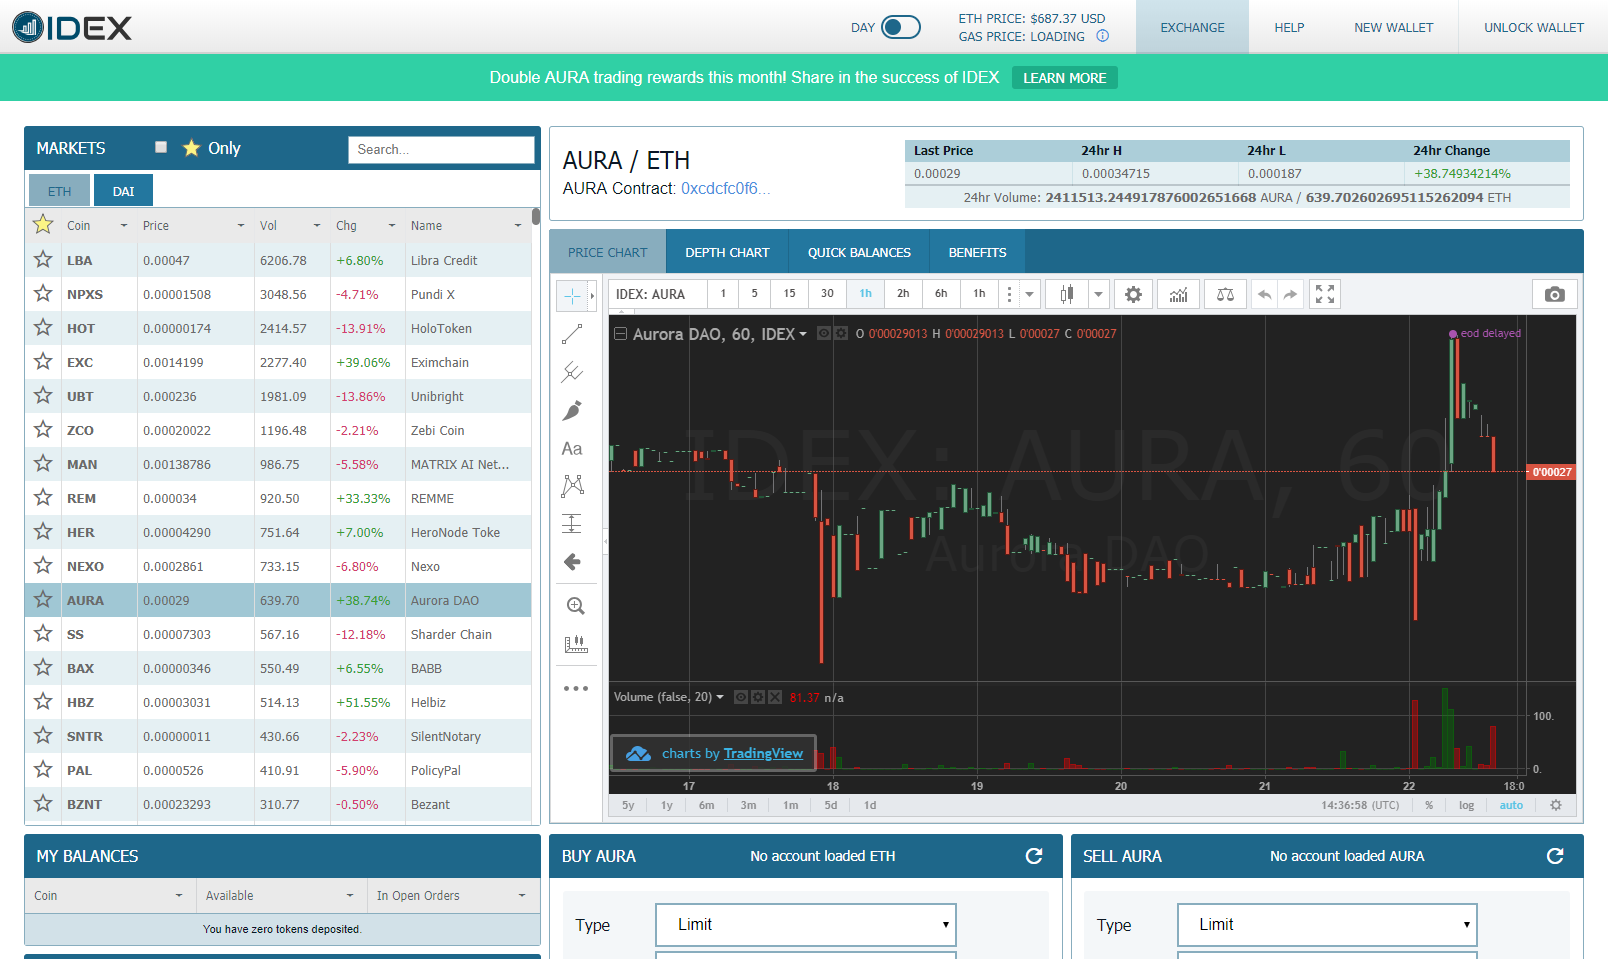
\includegraphics[width=\textwidth]{idex}
    \caption{Front page of the IDEX trading platform}
    \label{fig:idex}
\end{figure}

There are numerous escrow services on the platform, but mostly, they only provide their services for Ether to Ether or token to token transactions. We also searched the State of the DApps platform for any DApps that would interact with real-world data. The most notable example is a flight-cancellation insurance provider Etherisc\footnotemark. They provide insurance on flight delays and cancellations, promising automated payout, shall the flight be deleted. On their website however, the possibility to engage in an insurance policy with Ether is currently disabled. The smart contract featured by Etherisc is on a Ropsten test network and we could not locate a contract on the mainnet, so the actual usage of this application could not be determined. If it does work however, it needs to learn flight status data for its execution.
% 
\footnotetext{\url{https://fdd.etherisc.com/}, accessed 22-05-2018}
